\usetikzlibrary{arrows,positioning}
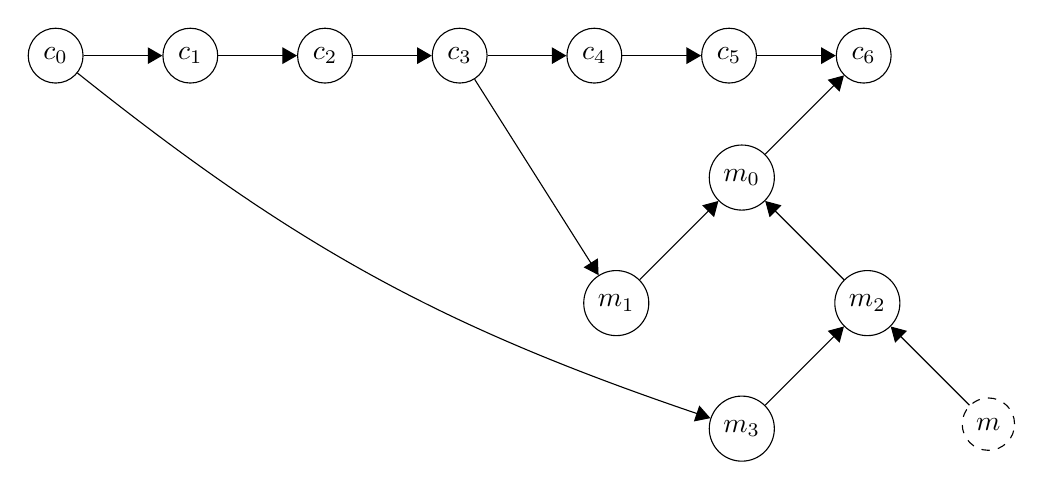
\begin{tikzpicture}[every node/.style={circle,draw},
                                    every path/.style={<-,>=triangle 60}]

\node (c0) {$c_0$};
\node[right=of c0] (c1) {$c_1$} edge (c0);
\node[right=of c1] (c2) {$c_2$} edge (c1);
\node[right=of c2] (c3) {$c_3$} edge (c2);
\node[right=of c3] (c4) {$c_4$} edge (c3);
\node[right=of c4] (c5) {$c_5$} edge (c4);
\node[right=of c5] (c6) {$c_6$} edge (c5);

\node[below left=of c6] (m0) {$m_0$} edge[->] (c6);
\node[below left=of m0] (m1) {$m_1$} edge[->] (m0) edge[<-] (c3);
\node[below right=of m0] (m2) {$m_2$} edge[->] (m0);

\node[below left=of m2] (m3) {$m_3$} edge[->] (m2) edge[bend left=10,<-] (c0);
\node[below right=of m2,dashed] (m4) {$m$} edge[->] (m2);


\end{tikzpicture}